\chapter{Grundlagen} 
\label{cha:Grundlagen}


\section{Java Virtual Machine} \label{sec:Java Virtual Machine}
  % java einleitung
  Gemessen am Interesse der Anwender und an seiner Verbreitung ist Java die erfolgreichste Programmiersprache der letzten Jahre. Der Erfolgt kam mit der Objektorientierung sowie der Plattformunabhängigkeit. Diese Fähigkeiten brachten eine große und fähige Kommune zusammen, die sowohl aus der Wirtschaft als auch aus der Forschungsbereich besteht. Dementsprechend ist Java im Laufe der Zeit durch Designmustern, Architekturkonzepten, Paradigmen und aktuellen Sicherheit- sowie Industriestandrats erweitert worden. 

  Da Renew mit Hilfe der Java Plattform umgesetzt wurde, kann sie sie sich alle gegebenen Vorteile zunutze machen. Einer der wichtigen Bausteine von Java ist die virtuelle Maschine, die das Suchen, Laden und Ausführen einer Codebasis auf allen gängigen Betriebssystemen erlaubt. Demzufolge spielt das Laden von Klassen aus Örtlich unabhängigen Plugins ein große Rolle für die entstandene Architektur. Die Plugins müssen gefunden, geladen und kommunikationsfähig eingerichtet werden, sodass sie sich gegenseitig nutzen und beeinflussen können.

  In diesem Kapitel werden grundlegende Konzepte des \textit{ Classpath's, Classloader's} und \textit{Reflection} erläutert mit Hilfe dessen die Renew Plugin-Architektur umgesetzt wurde.

\section{Classpath}\label{sub:Classpath}
  % classpath einleitung
  Jede Java-Anwendung wird zuerst in einer für menschlich verständlichen Sprache geschrieben und anschließend in ByteCode übersetzt. In Folge dessen ist der Code einsatzbereit für die Ausführung und wird an die virtuelle Maschine weiter gereicht.

  Um die compilierten Klassen zu laden, wird von der Java Virtual Machine Ortsangaben mit entsprechenden Code erwartet. Die Ortsangaben nennt man \textit{Classapth} oder Klassenpfad. Dieser beschreibt eine Liste von Orten an denen sich die zur Ausführung benötigten Klassen befinden, wie zum Beispiel das lokalen Dateisystem, das Netzwerk oder sogar die Datenbank. 

  Nachdem der Klassenpfad für die entsprechenden Classloader gesetzt ist, kann das \textit{Classlaoder System} die gewünschten Klassen erfassen und in die virtuelle Maschine laden.

  % simple classloader image 
  \begin{figure}[h]
    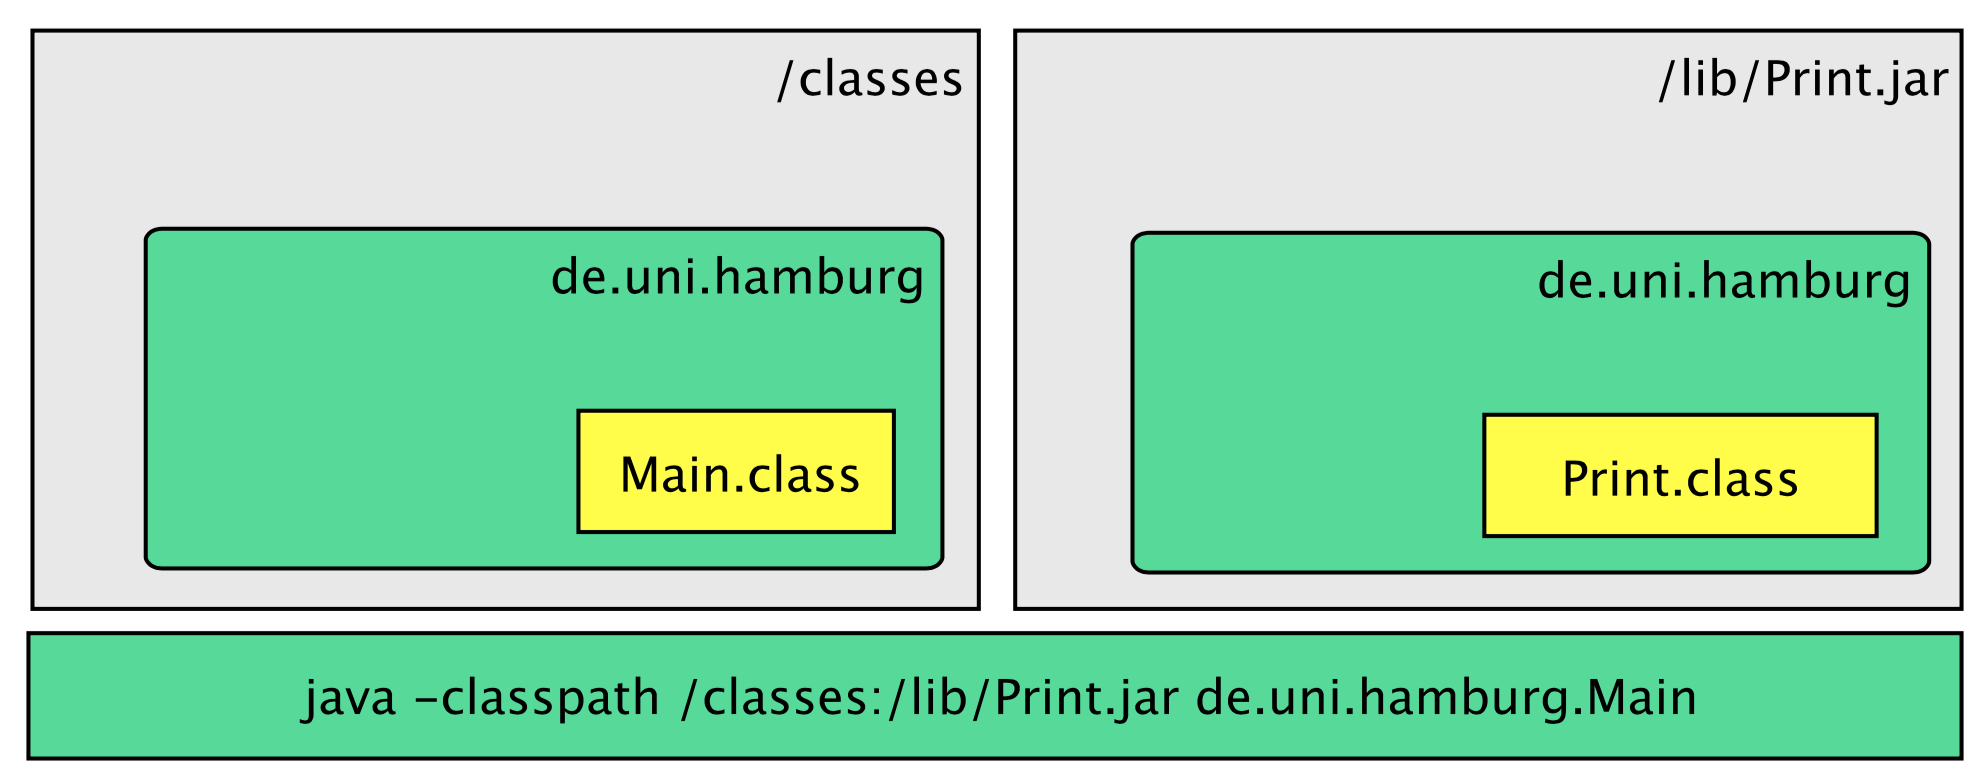
\includegraphics[width=\textwidth]{material/images/Classpath.png}
    \caption{Java Classpath}
    \label{fig:Classpath-Simple}
  \end{figure}

  % simple classloading 
  In Beispiel \ref{fig:Classpath-Simple} besteht der Klassenpfad aus einem Ordner sowie einem JAR-Archive, die für die Ausführung nötige Klassen beinhalten. Da beide Orte eine Dateistruktur beinhalten unterliegen sie einer Einschränkung: beide müssen die Paketstruktur der Java Klassen widerspiegeln damit der \textit{Applikation Classloader} diese durchsuchen kann. 

  Abschließend braucht Java einen Startpunkt, mit dem die Applikation ihre Ausführung beginnt. Jedes mal wenn eine Klasse instantiiert werden muss, wird der Klassenpfad von Links nach Rechts nach dem benötigten Typ durchsucht und instantiiert. Somit hat der Klassenpfad eine interne Ordnung und eine Abarbeitungsreihenfolge.
  \begin{figure}[h]
    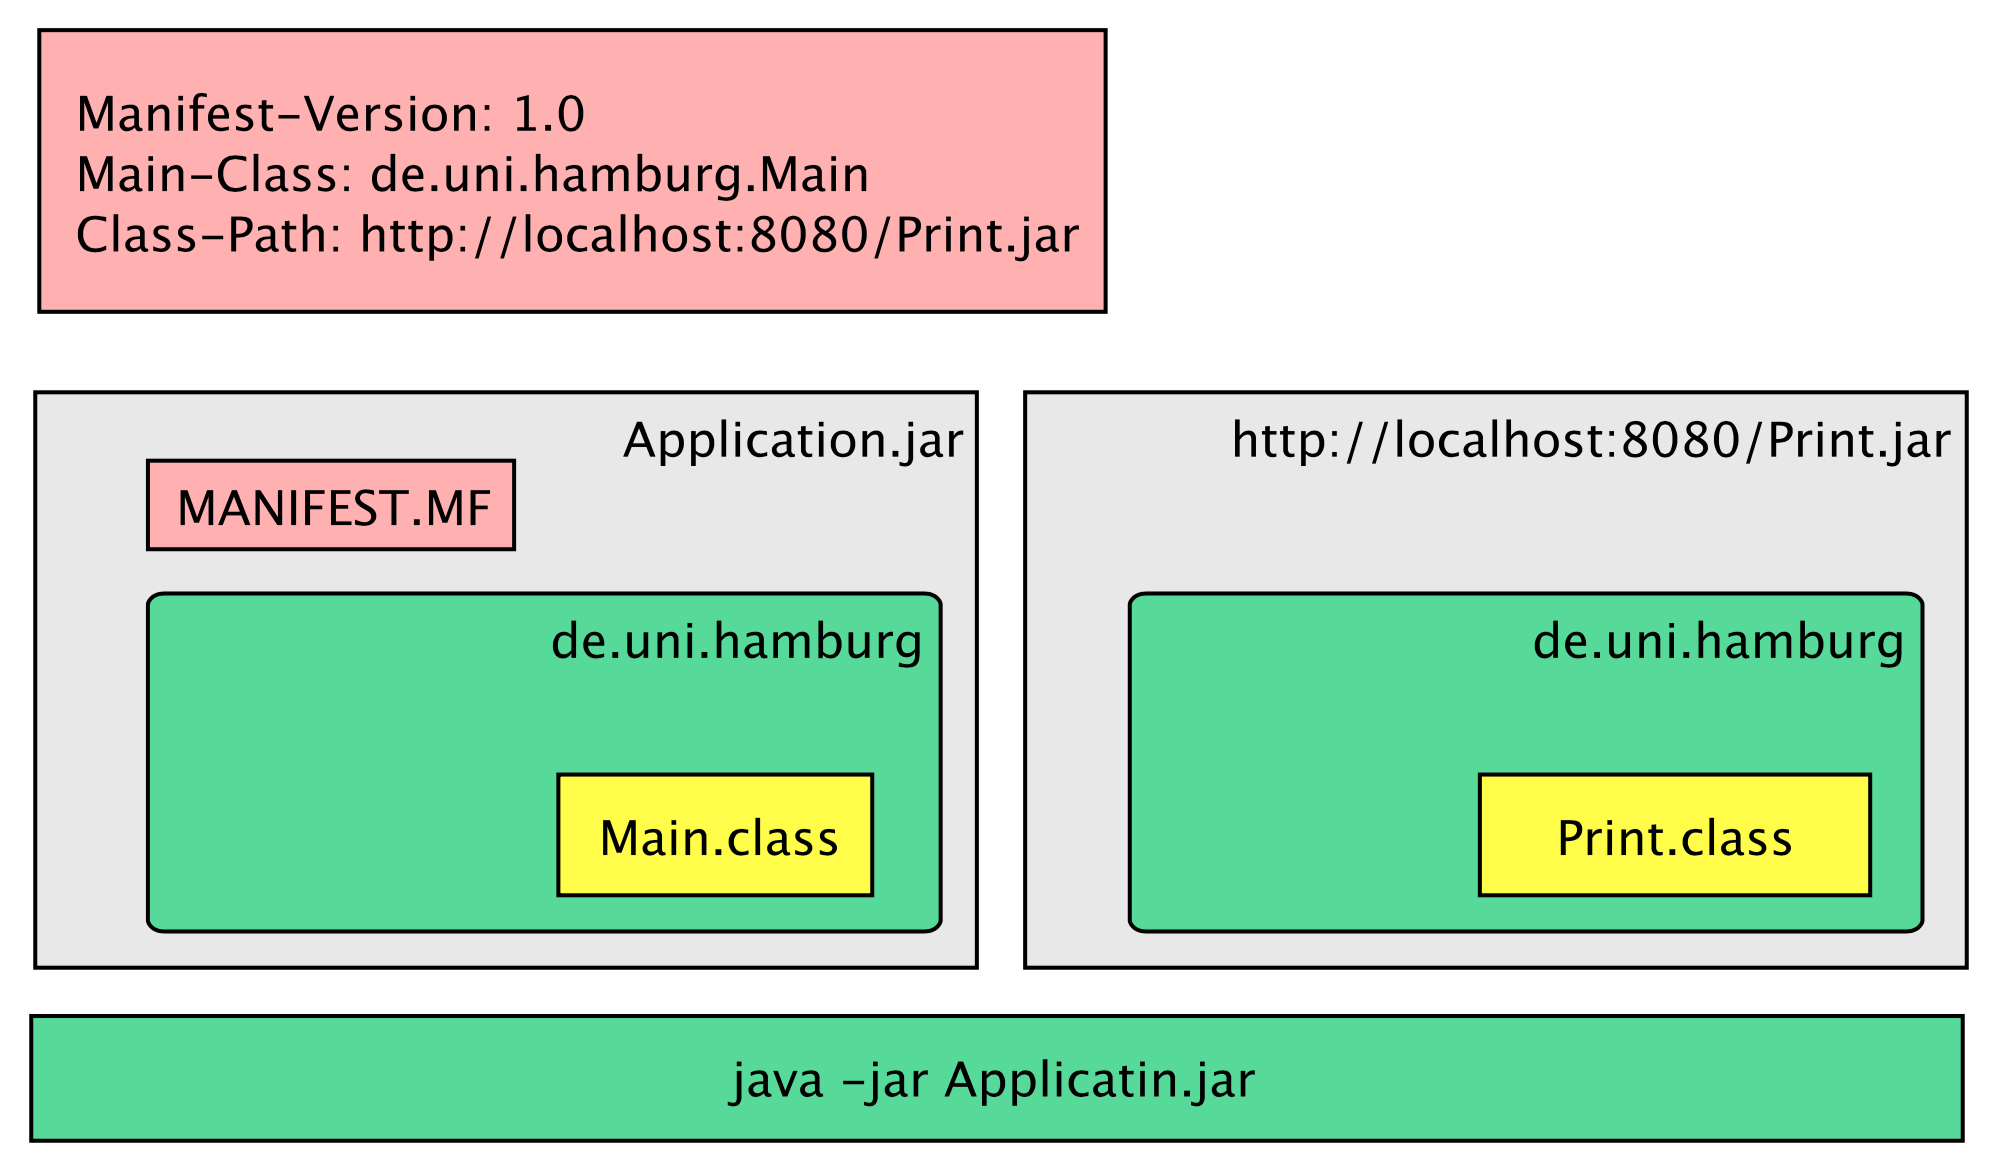
\includegraphics[width=\textwidth]{material/images/Classpath-Manifest.png}
    \caption{Jar Classpath}
    \label{fig:Classpath-Advanced}
  \end{figure}

  % jar classloading with manifest 
  Im Beispiel \ref{fig:Classpath-Simple} wurde explizit ein Applikationsklassenpfad gesetzt, der für die Ausführung benötigten Klassen zuständig ist. Für den Ablauf großer Applikationen mit viele Abhängigkeiten kann dieser ausgedehnt und chaotisch werden. Von daher bietet Java eine Archivstruktur, die einen standardisierten Aufbau sowie zusätzliche Meta-Information über den Container in sich trägt. 
  
  Mit Hilfe der Strukturrichtlinie befindet sich der komplette Inhalt eines Archivs auf dem Applikationsklassenpfad und kann zusätzlich in der \textit{manifest.mf} Datei erweitert werden. Die \textit{manifest.mf} spielt eine große rolle in der Entwicklung von Java Applikation, diese kann den Namen, die Version, den Entwickler und die Sicherheitsattribute tragen, die während der Laufzeit ausgewertet werden können. Zum Beispiel wird in \ref{fig:Classpath-Advanced} der Klassenpfad durch ein Archive aus dem web erweitert und für die Ausführung genutzt. Des weiteren hält die \textit{manifest.mf} einen Einstiegspunkt für die Ausführung, der auf eine Klasse mit der \textit{main Methode} verweist.
  
  Somit kann die Applikation in einer kurzen und einfachen Form gestartet werden, da der Ausführungskontext durch die Struktur und die mitgelieferten Meta-Information komplett ist.

\section{Classloader}\label{sub:classloader}
  In den vorherigen Beispielen [\ref{fig:Classpath-Simple}, \ref{fig:Classpath-Advanced}] wurde die Bedeutung und die Rolle des Klassenpfads für die Applikation beschrieben, dennoch muss dieser zuerst verarbeitet werden. Diese Aufgabe wird von dem Classloader übernommen, der eine zentrale Rolle in jeder Applikation spielt. Zumal er nach benötigten Java Klassen für die Instantiierung der entsprechenden Typen sucht. Da es eine wichtige Aufgabe ist, wird die Verantwortung für das Laden der Klassen über eine Menge von Classloader aus dem \textit{Classloader System} aufgeteilt. 

  \subsection{Classloader System} \label{sec:cls}
    Das \textit{Classloader System} besteht aus drei integrierte Classloader, von denen jeder einen anderen Gültigkeitsbereich für das Laden der Klassen besitzt. Beim Abstieg der Hierarchie wird der Umfang der verfügbaren Quellen breiter und weniger vertrauenswürdig. 
    %Die Idee hinter dem Separieren der Aufenthaltsorte ist, dass den Quellen unterschiedliche Vertrauensebenen zugewiesen werden können.
    \begin{figure}[h!]
      \centering
      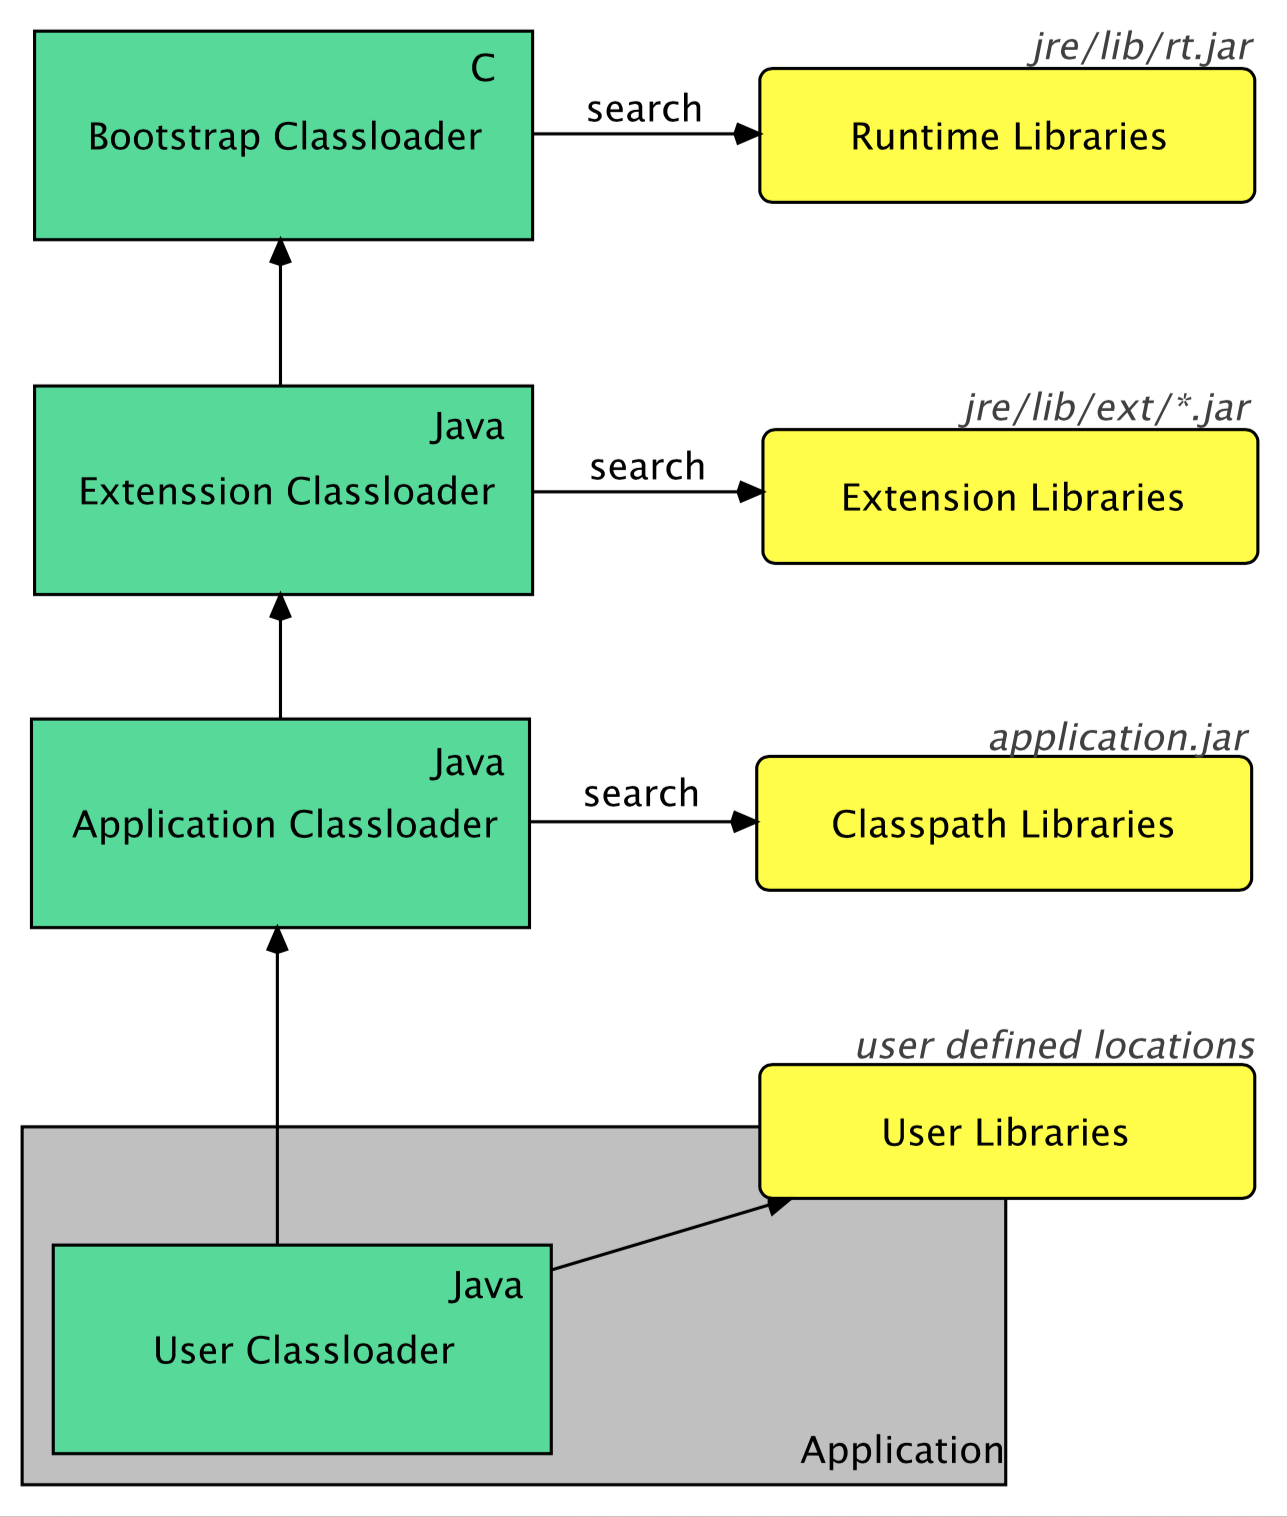
\includegraphics[width=0.7\textwidth]{material/images/Classloader.png}
      \caption{Classloader System}
      \label{fig:Classloader}
    \end{figure}
    
    Oben in der Hierarchie befindet sich der \textit{Bootstrap-Classloader}. Dieser Classloader ist verantwortlich für das Laden der grundlegenden Java Klassenbibliothek, wie die zum Beispiel Java-Core-API aus der \textit{rt.jar}. Diese Klassen sind am vertrauenswürdigsten und werden zum Starten der virtuellen Maschine verwendet. Der Classloader für Erweiterungen kann Klassen laden, die Standarderweiterungspakete im Erweiterungsverzeichnis \textit{lib/ext} sich befinden. Diese können Java-UI wie kryptografische Erweiterungen beinhalten. Der darunter liegende \textit{Applikation Classloader} ist zuständig für unseren Code und lädt Klassen aus dem allgemeinen Klassenpfad einschließlich der zu startenden Anwendung. Zuletzt können Benutzerdefinierte \textit{Classloader} erstellt werden, die sich auf der unteren Ebene der Classloader-Hierarchie befinden und auf Drittanbieter Bibliotheken zugreifen können. Demzufolge sind diese Quellen nicht sicher genug um ihnen große Priorität zuzuweisen, wie zum Beispiel den geladenen Klassen des \textit{Bootstrap-Classloader}. \bigbreak 

    Das in \ref{fig:Classloader} abgebildete Classloader System verhindert, dass Code aus weniger sicheren Quellen vertrauenswürdige Core-API-Klassen ersetzt, indem der selbe Name als Teil der Core-API angenommen wird. Daraus folgt ein Delegierungsmodell, welcher eindeutige Klassen garantiert, da die Klassensuche von Oben nach Unten der Classloader-Hierarchie abgearbeitet wird. 
    
  \subsection{Delegierungsmodell}
    Das \textit{Classloader System} delegiert jede Anfrage zum Laden einer bestimmten Klasse zuerst an seinen übergeordneten Classloader, bevor der angeforderte Classloader versucht die Klasse selbst zu laden. Jeder Classloader hält somit einen Verweis auf einen übergeordneten Classloader und ist Teil eines Classloader Baums mit dem \textit{Bootstrap-Classloader} an der Wurzel. 

    Wenn eine Instanz einer bestimmten Klasse benötigt wird, prüft der Classloader, der die Anfrage bearbeitet, normalerweise mit seinem übergeordneten Classloader vorab. Der übergeordnete Classloader durchläuft wiederum den gleichen Prozess bis die Delegierungskette den \textit{Bootstrap-Classloader} erreicht. Sobald der \textit{Bootstrap-Classloader} erreicht wurde, beginnt die tatsächliche Suche nach der gewünschten Klasse.
    \begin{figure}[h]
      \centering
      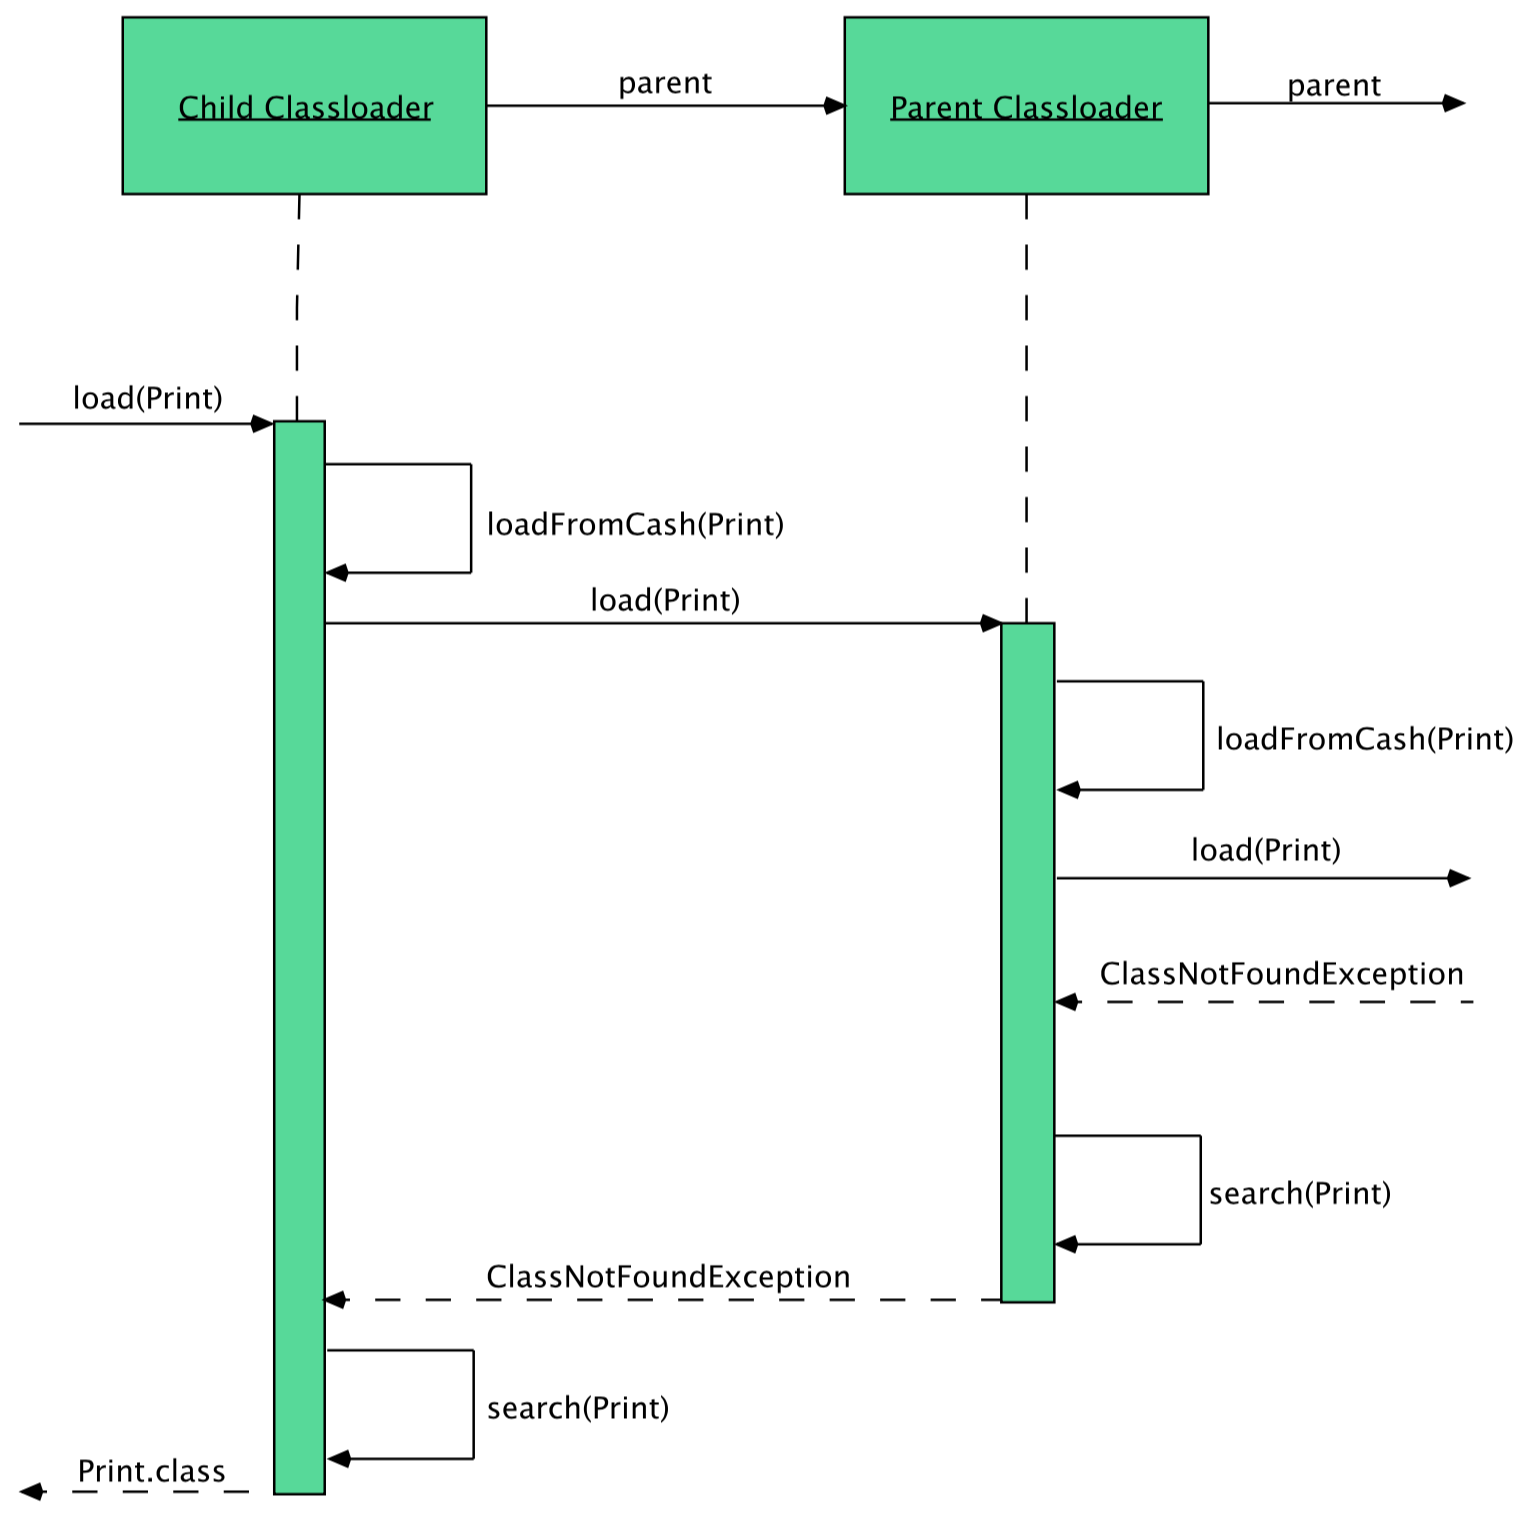
\includegraphics[width=0.9\textwidth]{material/images/deligation.png}
      \caption{Klassensuche}
      \label{fig:deligation}
    \end{figure}

    Wenn während der Suche ein übergeordneter Knoten eine bestimmte Klasse findet, dann wird diese Klasse die Baumhierarchie herunter zu der Anfrage delegiert. Andernfalls versucht der zuständige Classloader als letzter die Klasse selbstständig zu laden. Dies bedeutet, dass eine Klasse normalerweise nicht nur in dem Classloader sichtbar ist, der sie geladen hat, sondern auch für alle untergeordneten Instanzen. Dies bedeutet auch, wenn eine Klasse von mehr als einem Classloader in einem Baum geladen werden kann, wird immer die Klasse des übergeordneten Classloader eingelesen.

    Dennoch wird vor jedem Laden der Klasse der Cash-Speicher des Classloaders nach der gewünschten Instanz durchsucht. Wenn diese existiert, wurde die Suche bereits zuvor durchgeführt und keiner der übergeordneten Classloader außer dem jetzigen, war fähig die Anfrage zu beantworten. Somit kann die Suche beschleunigt werden, indem der Type sofort zurückgegeben wird.

  \subsection{Namensräume} \label{sec:Namensräume}
    Geladene Klassen werden sowohl durch den Klassennamen als auch durch den Classloader eindeutig identifiziert. Demzufolge werden geladene Klassen in \textit{Namensräume} unterteilt, die vom \textit{Classloader System} individuell behandelt werden.

    Ein \textit{Namensraum} ist eine Gruppe von Klassennamen, die von einem bestimmten Classloader geladen worden ist. Wenn ein Eintrag für eine Klasse einem \textit{Namensraum} hinzugefügt wurde, ist es nicht möglich, eine andere Klasse mit dem selben Namen und unterschiedlichen Inhalt in den gleichen \textit{Namensraum} einzubinden. 

    Nichtsdestotrotz können mehrere Kopien einer beliebigen Klasse in die Applikation geladen werden, indem für jede Klasse ein Classloader mit dem separaten \textit{Namensraum} erstellt wird. 
    \begin{figure}[h]
      \centering
      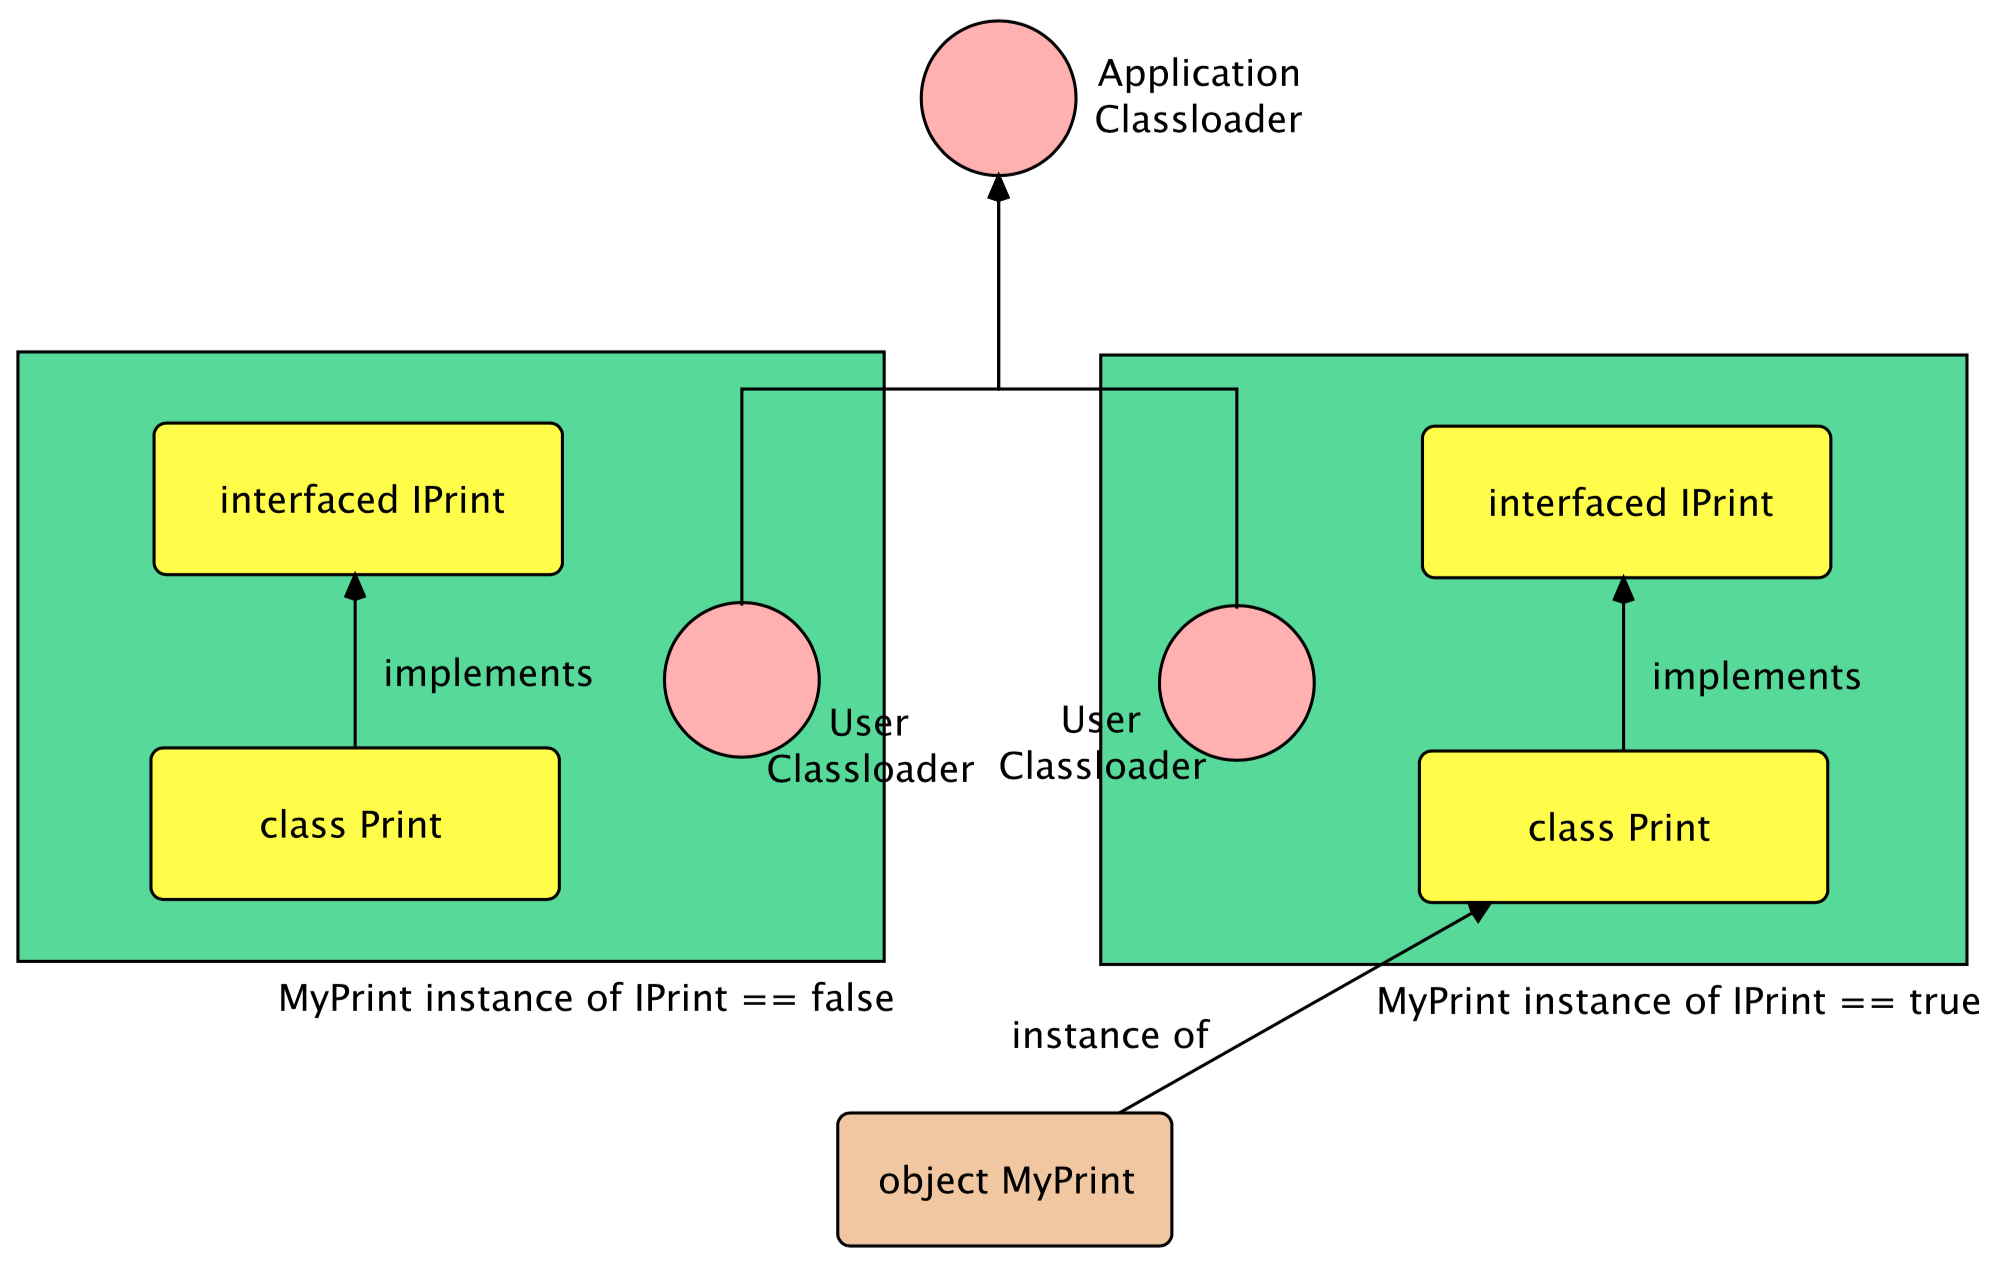
\includegraphics[width=0.9\textwidth]{material/images/namespaces.png}
      \caption{Namensräume}
      \label{fig:namespaces}
    \end{figure}

    Die Abbildung \ref{fig:namespaces} zeigt ein Beispiel für eine Klassenidentitätskrise, die sich ergibt, wenn eine Schnittstelle und die zugehörige Implementierung jeweils von zwei separaten Classloader geladen werden. Obwohl die Namen und binären Implementierungen der Schnittstellen und Klassen gleich sind, kann eine Instanz der Klasse von einem Classloader nicht als Implementierung des Interfaces von dem anderen Classloader erkannt werden.

    Bei Wunsch kann dieser Umstand gelöst werden, indem das Interface eine Ebene höher rutscht und von den Applikation Classloader geladen wird. Somit implementieren beide \textit{Print} Klassen die selbe Schnittstelle.\bigbreak 

    Der Klassen Namensraum bieten zusätzliche Sicherheitsfunktionen wie die Kapselung privat deklarierter Pakete. Die Namensräume verhindern, dass weniger vertrauenswürdiger Code, der aus der Applikation oder benutzerdefinierte Classloader geladen worden ist, direkt mit mehr vertrauenswürdigen Klassen interagieren kann. Beispielsweise wird die Kern-API vom \textit{Bootstrap-Classloader} geladen, diese kann \textit{package private} Code enthalten, der bei Anfrage nicht an die unterliegende Classloader weitergereicht wird.

    Auch wenn ein untergeordneter Classloader die Paketstruktur der Core-API nachahmt, wird diese nicht als Teil der Java Core-API anerkannt, da dieser von den falschen Classloader geladen wurde. Somit verhindert die Verwendung von Namensräumen die Möglichkeit spezielle Zugriffsberechtigungen auf private Pakete zu erhalten, indem man selbst geschriebenen Code diesen zuweist.

\section{Schnittellen} \label{sub:Kapselung}
  Die Schnittstelle und dessen Implementierung spielt eine entscheide Rolle für das Nutzen der Klassenfähigkeit. Eine Schnittstelle ist ein Vertrag, die die Funktionalität alle Klassen, die dieses implementieren beschreibt. Wenn eine Klasse eine bestimmte Schnittstelle implementiert, verspricht sie die Umsetzung aller in der Schnittstelle deklarierten Methoden.

  \begin{figure}[h!]
    \centering
    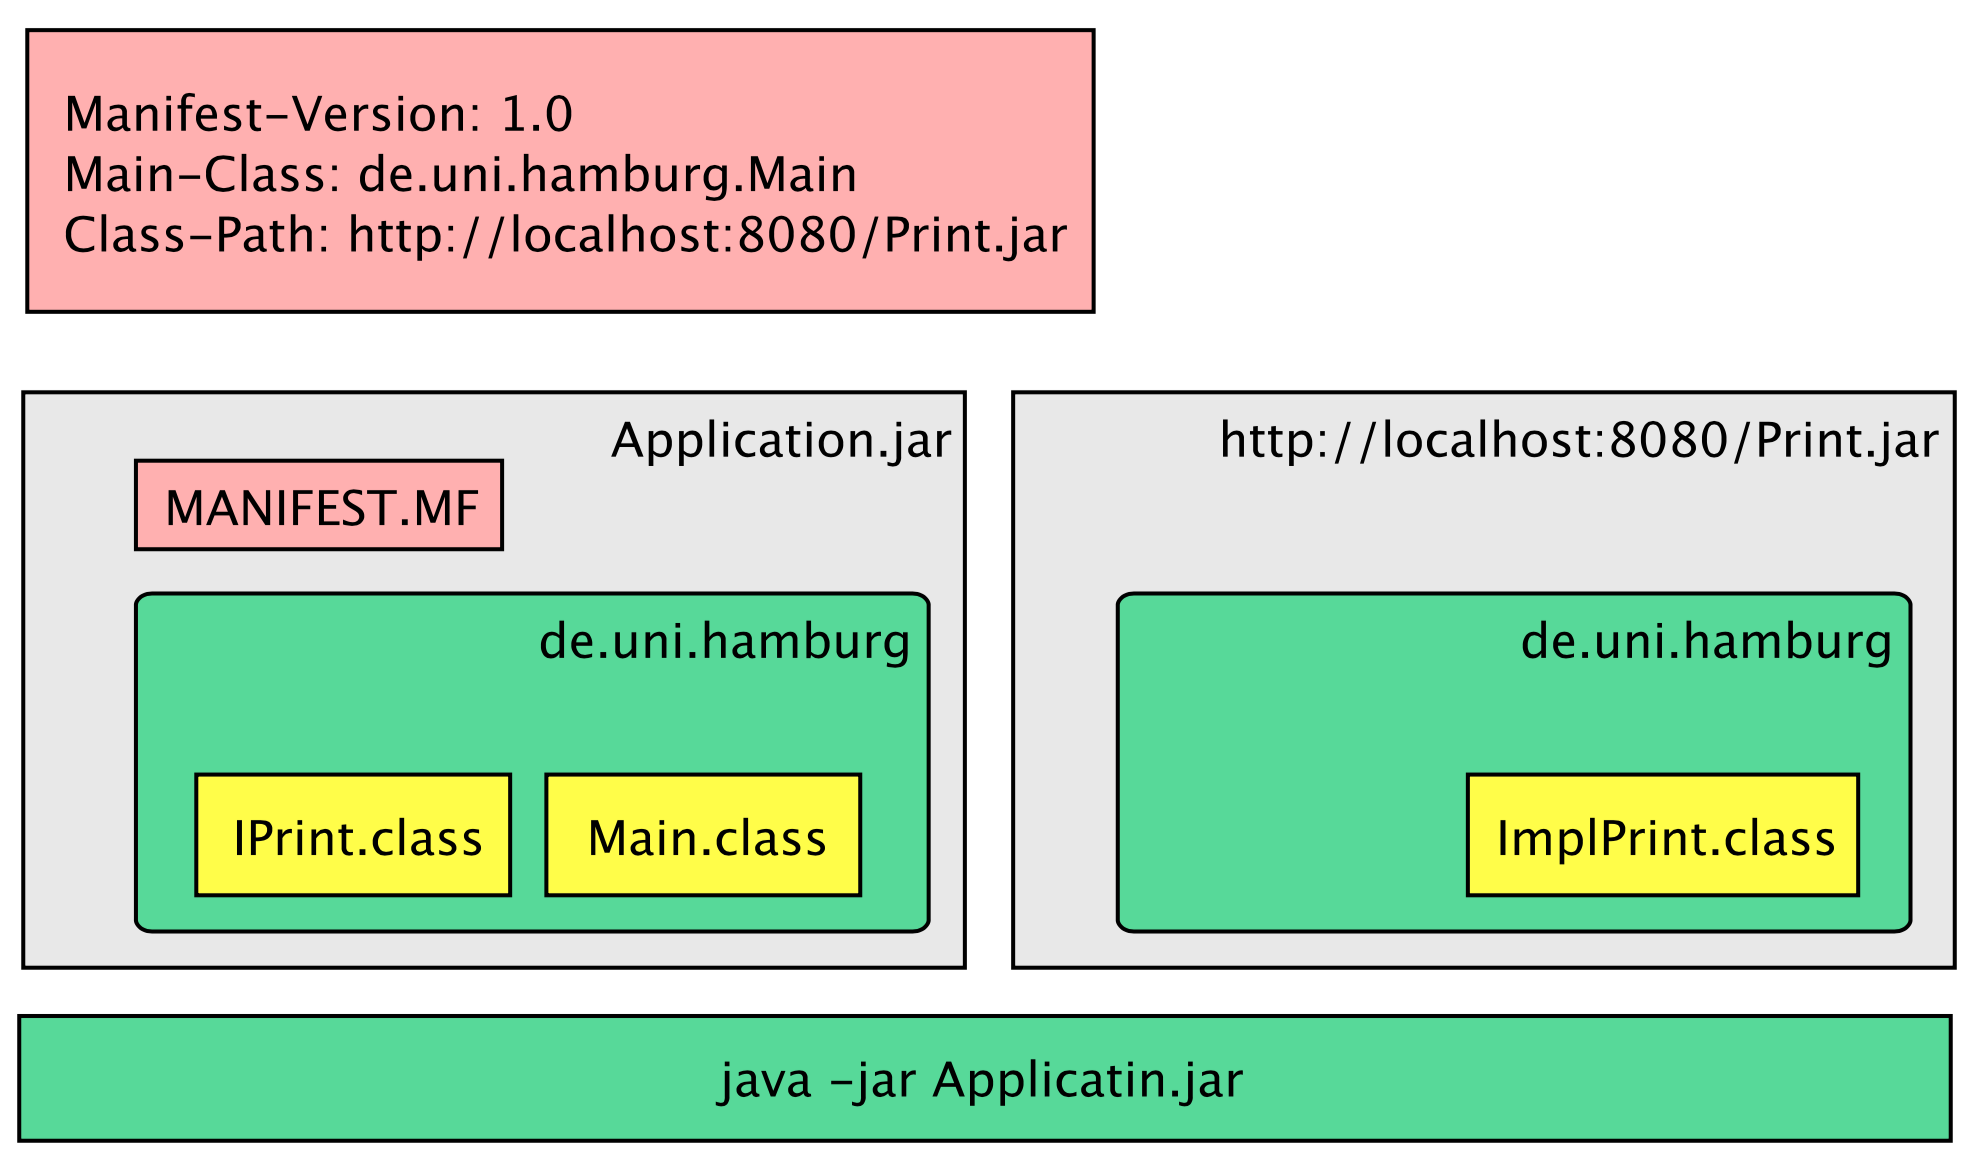
\includegraphics[width=0.8\textwidth]{material/images/Interface.png}
    \caption{Schnittstelle}
    \label{fig:Schnittstelle}
  \end{figure}

  Somit wird durch die eigene Umsetzung des Schnittstellenvertrags eine mögliches Verhalten für die Nutzer der Schnittstellenbeschreibung implementiert. Daraus folgt ein Kommunikationsvertrag zwischen zwei Objekten, denn wenn eine Klassen eine Schnittstelle implementiert, implementiert diese alle in dieser Schnittstelle deklarierten Methoden und der Methodenaufruf an dieser Klasse wird garantiert ausgeführt.\bigbreak 
  
  Im Beispiel \ref{fig:Schnittstelle} wird der Vorteil des Schnittstellenvertrags demonstriert, der das Ausführen, für die Applikation unbekannte \textit{PrintImpl} Umsetzung, durch eine einfache Schnittstellenbeschreibung \textit{IPrint} garantiert. Solange die Implementation sich auf der selben Klassenpfadhierarchie befindet wie die Schnittstelle, wird diese während der Laufzeit auf Kompatibilität geprüft und angewandt. Somit kann dynamische Klassenbindungen während der Laufzeit entstehen und Laufzeitbibliotheken ausgetauscht werden ohne die Applikation zu verändern. Hätte man die Schnittstelle nicht genutzt, würde man die Implementation nur als ein Objekt Type instantiieren können und hätte keinen einfachen Zugriff auf ihre Methoden. In der Konsequenz verbirgt die Schnittstelle ihre Implementierungsdetails der Methoden und gewährt den Vertragspartner keinen Einblick ihn ihre Umsetzung. Daraus folgt eine einfache Ersetzbarkeit der Implementationsvertreter ohne den Klienten anpassen zu müssen.  

\section{Reflection}\label{sec:reflaction}
  % Kurze einleitung 
  Reflection ist die Fähigkeit eines laufenden Programms, sich selbst und seine Softwareumgebung zu analysieren und zu ändern. 
  Somit hat die Applikation eine Möglichkeit, durch Reflexion, die Information über ihre Struktur und ihr Verhalten zu erhalten, um wichtige Entscheidungen zu treffen.

  Je nachdem welche Information durch die Untersuchung eigener Klassen ausgelesen wurde, können Objekte, die während der Kompilierung nicht präsent waren, mit Hilfe der Reflection-API während der Laufzeit instantiiert, bearbeitet und genutzt werden. Somit ermöglicht Reflection das Arbeiten mit Klassen von den man im Voraus nicht wissen kann, wie zum Beispiel von Klassen, die in der Zeit nach der Applikation entstanden sind.\bigbreak 

 % Überblick: Problemstellung die Reflexion löst 
  In vielen Fällen der Applikationsentwicklung möchte man seinen Applikation von andren Nutzern und Entwicklern erweitern lassen, ohne das diese bei jeder Änderungen die komplette Applikation umbauen. Somit stellt sich die Frage, wie erstellt man ein Mechanismus der mit beliebigen Klassen arbeiten kann. Man könnte mit dem zuvor vorgestellten Schnittstellen- und Implementierungsansatz eine gemeinsame Schnittstelle für Erweiterungen definieren, die unserer Applikation mit einer Implementation erweitern lässt und die entsprechenden Methoden definiert. Nichtsdestotrotz besteht die Applikation nicht nur aus unserem Code, sondern zusätzlich aus Kern und Drittanbieter Bibliotheken über die wir keine Kontrolle verfügen. Somit ist die Erweiterung der gesamten Codebasis mit der entsprechenden Schnittstelle oder eine Verschachtlung von \textit{instanceof} Blöcken keine simple oder saubere Lösung. 

  Dementsprechend sollte Reflection genutzt werden, diese ermöglicht den Einblick in die Klassenstruktur ohne direkten den Typen zu kennen. Die Klassenstruktur enthalten Informationen über die Klasse selbst, z. B. das Paket und die Superklasse der Klasse sowie die von der Klasse implementierten Schnittstellen. Es enthält auch Details zu den von der Klasse definierten Konstruktoren, Feldern und Methoden.\bigbreak

  % Sequenzdiagram 
  In der Abbildung \ref{fig:reflection-fluss} wird ein Ablauf eines Methodenaufrufs mit Hilfe von Reflection visualisiert. Im ersten Schritt muss die Methode gefunden werden. Da wir den Typen nicht kennen und nur des Objekt Typs deklarieren Methoden nutzen können, lassen wir das Objekt sich selbst inspizieren und die geforderte Methode finden. Dafür wird nach einer bestimmten Methode der Klasse gesucht und bei Erfolg ein Objekt von Typ \textit{Method} zurückgegeben. 

  Das Methodenobjekt enthält die ganze Information über die gesuchte Methode, wie zum Beispiel Parameter und Rückgabewerte. Ausgerüstet mit der benötigten Information, kann die Methode ausgeführt werden. Dafür braucht das Methodenobjekt eine Instanz der passenden Klasse sowie für die Ausführung benötigten Parameter. 

  Nach der Abwickelung wird das Ergebnis der Ausführung vom der Objektinstanz über das Methodenobjekt zurück in den Programmfluss delegiert. 

  \begin{figure}[h!]
    \centering
    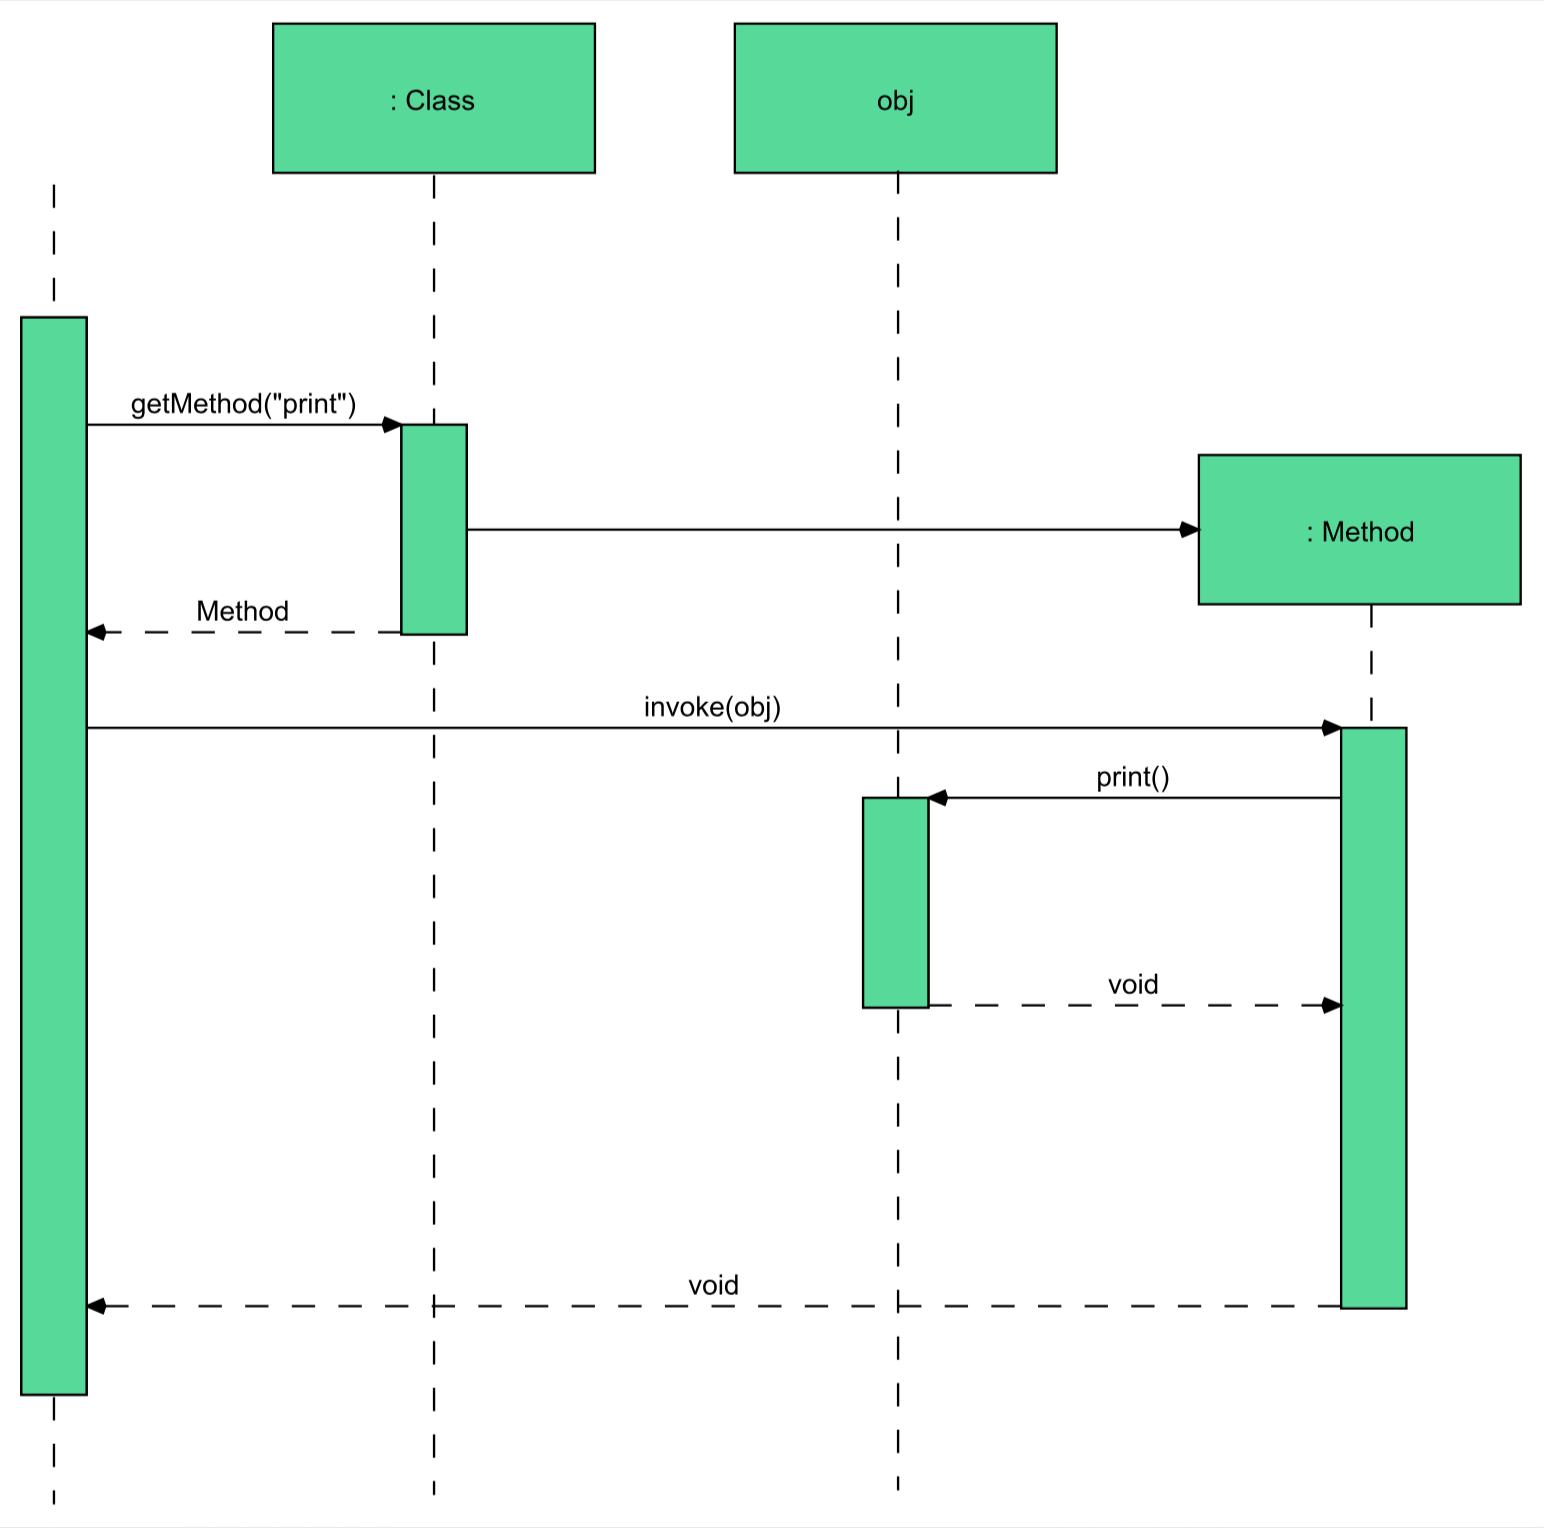
\includegraphics[width=0.8\textwidth]{material/images/reflection-flussdiagram.png}
    \caption{Aufruf einer Methode}
    \label{fig:reflection-fluss}
  \end{figure}

 % Nutzen: Felder Methode, Konstruktoren
  \newpage Somit sind die drei Hauptmerkmale einer Klasse ihre Felder, Methoden wie Konstruktoren durch eine entsprechendes Java Objekt aus der Reflection-API repräsentiert. 
  \begin{itemize}
    \item java.lang.reflect.Field
    \item java.lang.reflect.Method
    \item java.lang.reflect.Constructor
  \end{itemize}
  Mit Hilfe der Klassen Objektes eines Typs können die oben genannten Objekte erzeugt und manipuliert werden. Diese bietet eine Schnittstelle für das Abfragen ihrer Struktur an den Nutzer und liefert ein Objekt aus dem \textit{java.lang.reflection} Paket zurück.
  \begin{itemize}
    \item Field[ ] *.class.getFields();
    \item Method[ ] *.class.getDeclaredMethods();
    \item Constructor[ ] *.class.getConstructors();
  \end{itemize}
  \bigbreak 

  Um den Zusammenhang und den Nutzen von Reflection darzustellen wird in der Abbildung \ref{my-Reflection} ein Szenario durchgespielt, das eine unbekannten Typen mit Hilfe des Konstruktors initialisiert, dessen Methoden aufruft, das Feld bearbeitet und wiedergibt, ohne die Objektstruktur im Voraus zu kennen. Des Weiteren ist zu beachten, dass statische Klassenmethoden sowie private Felder und Methoden mit Hilfe von Reflection offen zugänglich gemacht werden können.\bigbreak 

  % Bild mit Code der eine Objekt erstellt und Methoden aufruft. Mit Kommentaren zwischen den Zeilen.
  \begin{lstlisting}[caption=Reflection in Aktion,label=my-Reflection,captionpos=b]
    public static void getMethods(@NotNull Class clazz) throws
            NoSuchMethodException, NoSuchFieldException,
           InvocationTargetException, InstantiationException,
           IllegalAccessException {
      Method method;

        // Instantiierung
        Constructor[] ctors = clazz.getDeclaredConstructors();
        Object dynamic = ctors[0].newInstance(4);
        // Aufruf einer privaten Methode
        method = clazz.getDeclaredMethod("print", String.class);
        method.setAccessible(true);
        method.invoke(dynamic,"Hello World");
        // Feld Manipulation
        Field field = clazz.getDeclaredField("version");
        field.set(dynamic, 5);
        int version = (int) field.get(dynamic);
        System.out.println(version);
    }
  \end{lstlisting}

 % Wo wird Reflection genutzt, wieso ist es so nützlich in der Modernen Software-Entwicklung 
  Wie in der Abbildung \ref{my-Reflection} dargestellt ist Reflection ein mächtiges Werkzeug, das aus der morden Softwareentwicklung nicht wegzudenken ist. Reflection wird in Framework's verwendet um den Entwickler zu unterstützen. 
  \begin{itemize}
    \item Zum Beispiel wird \textit{Dependency Injection} mit Hilfe von Reflection realisiert, indem das Framework (Spring) die entsprechenden Implementierung für ein Interface sucht und initiiert. In Diesem Zusammenhang wird Anhand des \textit{implement} Schlüssels und zusätzlicher Meta-Information aus der Klassen \textit{Annotation} ein eindeutiger Kandidat auserwählt und konstruiert.
    \item Beim Serialisieren und Deserialisieren von Objekten werden die Objektfelder in JSON und wieder zurück konvertiert, ohne die Feldnamen sowie ihre Anzahl zu kennen.
    \item Der Web-Container wie Tomcat oder WildFly leiteten die Web-Anfragen an das entsprechenden Module durch das Analysieren der \textit{web.xml} und Anfordern der passenden URI.
    \item JUnit verwendet Reflection, um die Methoden einer Klasse nach Test-Annotation zu durchsuchen, um diesen anschließend aufzurufen.
  \end{itemize}



% \subsubsection{OSGi}


% \subsubsection{Docker}
% \subsubsection{JavaScript}
% \subsubsection{TypeScript}
% \subsection{Java Umsetzung} 
% % wie es war mit 1.8
% % was draus gewirden ist in 9
% \newpage

% \section{Vergleich mit anderen Modularisierungskonzepten}


% \subsection{Jigsaw}
% % wie löst java 9 die Probleme 
% % theoretisch 
% \subsection{Modular JDK}
% % bevor entwickler modularisieren muss da System selbst modular sein.
% % eine beispiel umsetzung
% % löst probleme von beginn an, praktische umsetzung 
% \subsection{Modulstruktur}
% % arten von modulen 
% % inhalt und aufbau
% % zugriffsberechtigungen 
% \subsection{Modulepfad}
% % classloader änderungen 
% % verweist nicht mehr auf klassen orte sondern auf  modul Orte
% \subsection{Optionale Abhängigkeiten}
% %  optionale erweiterbarkeit
% \subsection{Reflection}
% %  sicherer und braucht explizite konfiguration 
% % zugriff auf  alle klassen nicht mehr möglich 
% \subsection{Services} 
% \subsection{Migration}

% \section{Vergleich mit anderen Modularisierungskonzepten}


% \section{Modularisierungskonzepten}

% \subsection{Java Plattform Module System}

% \subsection{Vergleich mit anderen Modularisierungskonzepten}

% \subsection{Vom Classpath zum Modulpath}

% \subsection{Arten von Jigsaw-Modulen}

% \subsection{Service-Provider und -Consumer}

% \subsection{Abhängigkeitsgraph mit Graphviz}


% - Module gabs schon lagne 
% - osg 
% - und und und 
% - angular 